\lecture{14}{13 Mar 2025}{10:10}
\section{Spline Interpolation}
\begin{definition}
    Piecewise Polynomial Approximation:  The lagrange and hermite are global interpolation schemes where 
    they work for all interpolation nodes. We consider local alternatives
\end{definition}
\begin{definition}
    Piecewise Linear Interpolation: Constructs a linear interpolation between each point
    \(\left[ x_i, x_{i+1}  \right] \) where each subinterval is a Lagrange interpolation
    \begin{figure}[H]
        \centering
        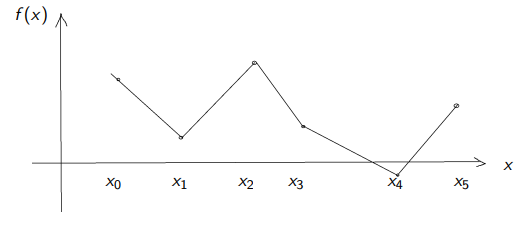
\includegraphics[width=0.5\textwidth]{Figures/03.png}
        \caption{}
        \label{fig:}
    \end{figure}
\end{definition}
\begin{definition}
    Piecewise Hermite Interpolation: Same as PLI but using a Hermite interpolation s.t. the polynomial is of 
    degree 3.
    \begin{figure}[H]
        \centering
        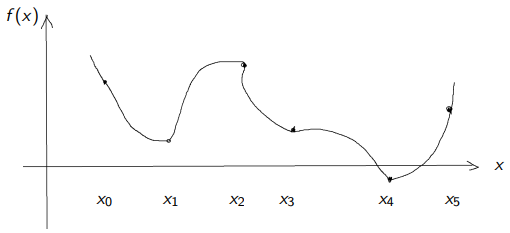
\includegraphics[width=0.5\textwidth]{Figures/04.png}
        \caption{}
        \label{fig:}
    \end{figure}
\end{definition}

What we wish for for a local interpolation has the following properties
\begin{enumerate}
    \item Smooth and differentiable at nodes
    \item One does not need the derivative to approximate \(f^{\prime} (x_i)\) 
\end{enumerate}
What we wish to find is the cubic spline interpolation. 
\begin{definition}
    Cubic Spline Interpolation: Given a function \(f\) defined with given nodes. The interpolant
    \(S(x)\) for \(f(x)\) satisfies the following conditions:
    \begin{enumerate}
        \item \(S(x)\) is a cubic polynomial 
        \item \(S_j (x_j) = f(x_j)\) and such for all points
        \item \(S_{j+1} (x_{j+1}) = S_j (x_{j+1} ) = f(x_{j+1} )\) 
        \item \(S^{\prime}_j = S^{\prime}_{j+1} \) 
        \item \(S_j ^{\prime\prime} = S_{j+1} ^{\prime\prime} \)
        \item The boundary conditions must be satisfied where either \(S^{\prime\prime} (x_0) = S^{\prime\prime} (x_n) = 0\)  or we must have that \(S^{\prime} (x_0) = f^{\prime} (x_0)\) and such for all other \(S^{\prime} \)  
    \end{enumerate}
\end{definition}

\begin{eg}
Suppose we have an example where we have the subintervals given as \(\left[ 1,2 \right] \)  and 
\(\left[ 2,3 \right] \)  
\begin{figure}[H]
    \centering
    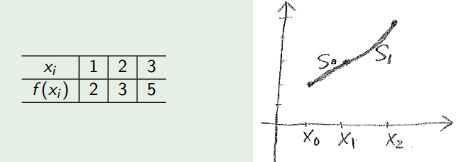
\includegraphics[width=0.5\textwidth]{Figures/05.png}
    \caption{}
    \label{fig:}
\end{figure}
which are given by the equation of the form
\[
    S_i (x) = a_i + b_i x + c_i x^{2}  + d_i x^{3} 
\]
where the index \(i\) denotes the equation. Given 8 unknowns from the two subintervals we have 8 equations to solve. 
\begin{enumerate}
    \item Match \(S_0 (x_0) = f(x_0) \) 
    \item Match \(S_0 (x_1) = f(x_1)\) 
    \item Next match the second line segment \(S_1\) to the B.C
    \item Match the first derivatives 
    \item Match the second derivatives
    \item Use the natural boundary condition at \(x_0\) and \(x_2\) where the second derivatives must be 0
\end{enumerate}
Satisfying these 8 conditions we can solve which gives us the cubic spline interpolant
\end{eg}
\begin{theorem}
    Uniquness of Natural Cubic Spline Interpolant: If \(f\) is defined for an interval 
    \(\left[ a,b \right] \) with points inside, \(f\) has a unique spline interpolant s.t. it satisfies the 
    natural B.C. s.t. \(S^{\prime\prime} (a) = S^{\prime\prime} (b) = 0\) 
\end{theorem}
From this we can define a general procedure to solve for the cubic spline. For notation, define
\(I_j = \left[  x_j, x_{j+1} \right]\)  for the \(j\)th interval. Then we have the segment as 
\[
    S_j (x0) = a_j + b_j (x- x_j) + c_j (x-x_j)^{2}  + d_j (x- x_j)^{3} 
\] 
Additionally define \(h_j = x_{j+1} - x_j \) 
The cubic spline is then written as 
\[
    S(x) = \begin{dcases}
        S_0(x), x \in I_0  ;\\
        \dots  \\
        S_{n-1}(x) ,x \in I_{n-1}   ;\\
    \end{dcases}
\]
\begin{enumerate}
    \item Fit the function on the nodes s.t. \(S_j(x_j) = f(x_j)\) where we are matching terms \(a_j = f(x_j)\) 
    \item Match interpolation on interior nodes for \(S_j (x_{j+1} ) = S_{j+1} (x_{j+1} ) \)  and so on s.t. we get 
    the form \(a_j + b_j h_j + c_j h_j ^{2}  + d_j h_j ^{3}  = a_{j+1} \) 
    \item Match the derivatives of the interior nodes where we must have 
    \(S_j^{\prime} (x_{j+1} ) = S_{j+1}^{\prime} (x_{j+1} ) \) which gives the form
    \[
        b_j + 2c_j h_j 3 d_j h_j ^{2}  = b_{j+1} 
    \]
    \item Match the second order derivatives at the interpolation nodes s.t. 
    \(S_j ^{\prime\prime}  (x_{j+1} ) = S_{j+1}^{\prime\prime} (x_{j+1} ) \) 
    which gives
    \[
        c_j + 3d_j h_j = c_{j+1} 
    \]
    \item Apply the natural boundary conditions s.t. \(S^{\prime\prime} (x_0) = 0 \implies  c_0 = 0\) 
    \item Apply the natural B.C. on the left s.t. \(S^{\prime\prime}_{n-1} (x_n) = 0 \)
    \[
        x_n = 0 \quad c_{n-1} + 3d_{n-1} h_{n-1} = 0 
    \] 
    Solve the coefficents to get that 
    \[
        d_j = \frac{1}{3h_j} \left( c_{j+1} - c_j \right) 
    \]
    \[
        a_{j+1} = a_j + b_j h_j + \frac{h_j ^{2} }{3}\left( 2c_j + c_{j+1}  \right) 
    \]
    \[
        b_{j+1} = b_j + h_j \left( c_j + c_{j+1}  \right) 
    \]
    Continuing the process, we can solve for all the necessary coefficients needed given the conditions solved. 
\end{enumerate}
\begin{remark}
    \begin{enumerate}
        \item We only find coefficients for \(S_j (0 \leq  j \leq  n-1)\) or the set 
        \( \left[ a,b,c,d \right] \) . the coefficient \(c_0 = 0\) is given by B.C. 
        \item Introducing extra variables isn't needed for the output of the algorithm, e.g. 
        \(a_n \equiv f(x_n), b_n = S^{\prime} (x_n), c_n = \frac{1}{2} S^{\prime\prime} (x_n)\) 
        \item Note that in the Natural B.C. case where \(c_n =0 \), \(b_n\) is undetermined but can be determined if 
        using the clamped B.C.
    \end{enumerate}
\end{remark}

The algorithm is given as shown below: 

\begin{algorithm}[H]
    \caption{Natural Cubic Spline}\label{alg:natural_cubic_spline}
    \KwIn{Integer $n$, arrays $x[0:n]$, $f[0:n]$}
    \BlankLine
    \textbf{Initialize:} \\
    $a[0:n] \gets 0$, $h[0:n-1] \gets 0$, $y[0:n] \gets 0$,\\
    $b[0:n-1] \gets 0$, $c[0:n] \gets 0$, $d[0:n-1] \gets 0$\;
    \BlankLine
    \For{$j=0$ \KwTo $n$}{
        $a[j] \gets f[j]$\;
    }
    \For{$j=0$ \KwTo $n-1$}{
        $h[j] \gets x[j+1] - x[j]$\;
    }
    \For{$j=1$ \KwTo $n-1$}{
        $y[j] \gets \dfrac{3}{h[j]}\Bigl(a[j+1]-a[j]\Bigr) - \dfrac{3}{h[j-1]}\Bigl(a[j]-a[j-1]\Bigr)$\;
    }
    \BlankLine
    \textbf{Initialize matrix} $A[0:n, 0:n] \gets 0$, with $A[0,0] \gets 1$ and $A[n,n] \gets 1$\;
    \For{$j=1$ \KwTo $n-1$}{
        $A[j,j-1] \gets h[j-1]$\; 
        $A[j,j] \gets 2\Bigl(h[j-1]+h[j]\Bigr)$\; 
        $A[j,j+1] \gets h[j]$\;
    }
    \BlankLine
    $c \gets \text{LinSolve}(A,y)$\;
    \For{$j=0$ \KwTo $n-1$}{
        $d[j] \gets \dfrac{1}{3h[j]}\Bigl(c[j+1]-c[j]\Bigr)$\;
    }
    \For{$j=0$ \KwTo $n-1$}{
        $b[j] \gets \dfrac{1}{h[j]}\Bigl(a[j+1]-a[j]\Bigr) - \dfrac{h[j]}{3}\Bigl(2c[j]+c[j+1]\Bigr)$\;
    }
    \BlankLine
    \Return $a,\, b,\, c,\, d$\;
    \end{algorithm}